\chapterimage{Week7Safety.png} 
\chapter{Safety}
\section{Hazard Control Approaches}\index{Hazard Control Approaches}
There are many hazards encountered in wastewater treatment operations.  
The three principal approaches for hazard control are:
\begin{itemize}
\item Engineering Controls:  Engineering controls include incorporating safety elements during engineering design and include considerations related to selecting a less hazardous alternatives, establishing  physical barriers and elements related to ventilation.
\item Administrative Controls:  Administrative controls are used to improve safety within the workplace by putting in place policies and rules that reduce the occupational risk faced by workers via altering the way their work is performed.  These include: housekeeping, materials handling and transfer procedures, training, providing facilities to support personal hygiene practices and medical surveillance.
\item Personal Protective Equipment: Personal protective equipment (PPE)is equipment worn to minimize exposure to hazards that cause serious workplace injuries and illnesses.  PPE includes respiratory protection and protective clothing - hard hats, safety
glasses/goggles, work gloves, chemical resistant gloves and safety shoes.

\end{itemize}


\section{Wastewater Treatment Hazards}\index{Wastewater Treatment Hazards}
\subsection{Hazardous Chemicals}\index{Hazardous Chemicals}
\begin{itemize}
\item Hazardous chemicals are used throughout wastewater treatment plants and in collection systems. 
\item To understand the dangers of these chemicals and to take adequate steps OSHA requires that the chemical manufacturer, distributor, or importer provide Safety Data Sheets (SDSs) (formerly MSDSs or Material Safety Data Sheets) for each hazardous chemical to downstream users to communicate information on hazards related to that particular chemical or product.
\item Employers must ensure that the SDSs are available and readily accessible to employees for all hazardous chemicals in their workplace.
\item The SDS includes information such as the properties of each chemical; the physical, health, and environmental health hazards; protective measures; and safety precautions for handling, storing, and transporting the chemical.\\
\end{itemize}


\subsubsection{Effects of Chemical Hazards}\index{Effects of Chemical Hazards}

Hazardous chemicals can cause:
\begin{itemize}
\item Headaches, rashes and burns
\item Respiratory problems
\item Lung and liver damage
\item Reproductive damage
\item Cancer
\item Death
\end{itemize} 


\subsubsection{Protection from chemicals}\index{Protection from chemicals}
Chemical manufacturers, distributors, or importers are required to provide Safety Data Sheets (SDSs) (formerly MSDSs or Material Safety Data Sheets) for each hazardous chemical to downstream users to communicate information on these hazards.
\begin{itemize}
\item Reading and understanding the associated Safety Data Sheets
\item Wearing appropriate Personal Protective Equipment
\item Implementing safe work practices by:
\begin{itemize}
\item \textbf{NEVER:} Eating, drinking or smoking when working with hazardous chemicals, and washing or storing PPE with personal clothing.
\item \textbf{ALWAYS:}Washing hands, arms and face with soap and water after use, ensuring integrity of PPE before and after use and also very importantly ensuring  readiness to deal with chemical exposure or spill.
\end{itemize}
\end{itemize}
\newpage
\hspace{0pt}
\vfill
\begin{center}
Safety Data Sheets Content - OSHA Guidance Document
\end{center}
\vfill
\hspace{0pt}
\pagebreak
\hspace{0pt}
\vfill
\begin{center}
\end{center}
\vfill
\hspace{0pt}
\pagebreak



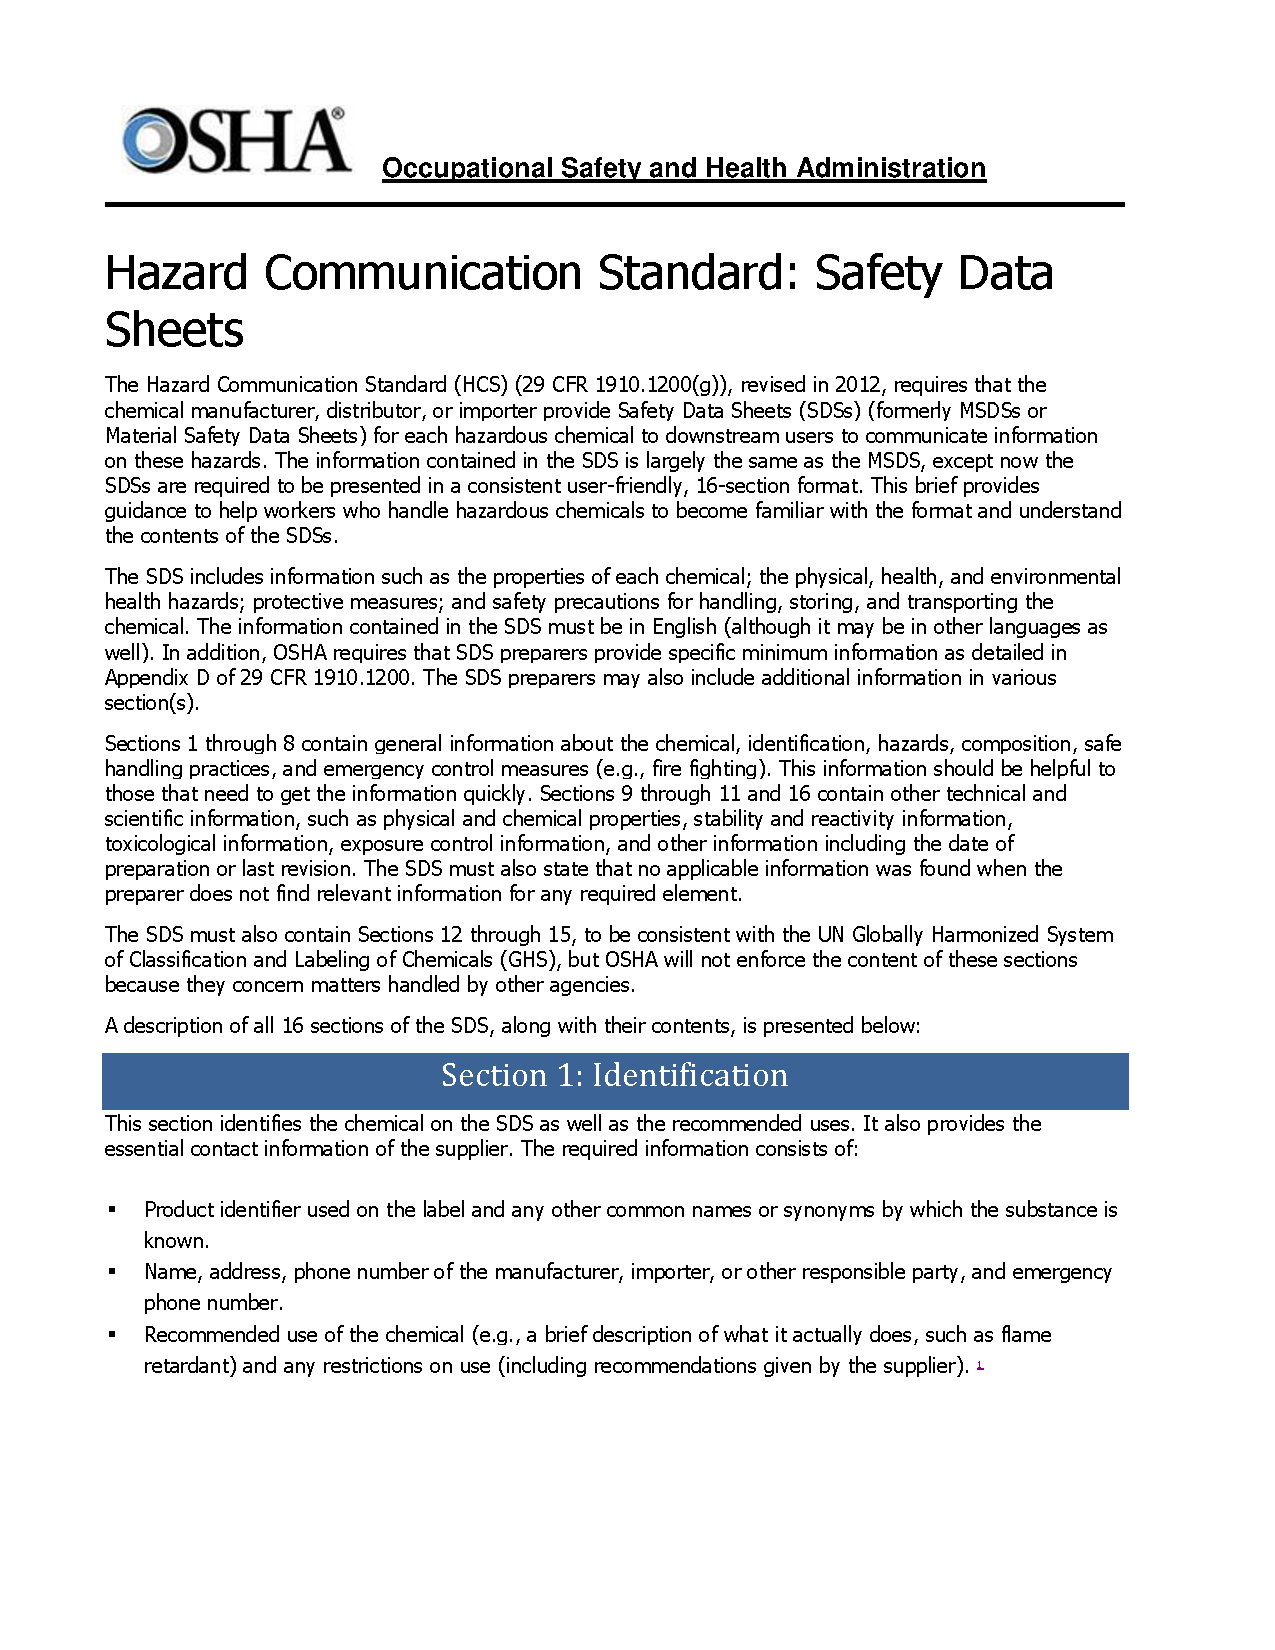
\includepdf[pages=-]{oshasds.pdf}
\newpage
\hspace{0pt}
\vfill
\begin{center}
Sample SDS
\end{center}
\vfill
\hspace{0pt}
\pagebreak
\hspace{0pt}
\vfill
\begin{center}
\end{center}
\vfill
\hspace{0pt}
\pagebreak
\includepdf[pages=-]{anhydammoniasds.pdf}

\subsection{Hazardous Gasses}\index{Hazardous Gasses}
\begin{itemize}
\item A summary of the properties and effects of hazardous gases found in wastewater operations is provided in the table below.
\item To safeguard against the potential impacts of these gases, employees are required to follow practices including donning appropriate Personal Protective Equipment (PPE) and utilizing respiratory protection\\
\end{itemize}
\begin{center}
\includegraphics[scale=0.6]{SafetyHazardousGases4}\\ 
\end{center}






\subsection{Falls}\index{Falls}
\begin{itemize}
\item Falls are one of the leading causes of injuries and deaths on the job.  Fall protection is a combination of methods and devices used to protect workers from falling off, onto, or through working levels. 
\item Fall protection methods and devices are typically divided into two categories: those that prevent falls and those that arrest falls. 
\item Examples of fall protection methods and devices include rails, guards, guardrails, barriers, fall-arrest systems, safety nets, hole covers, and various work practices and procedures.
\end{itemize}
\begin{center}
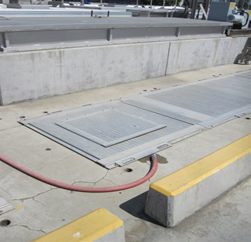
\includegraphics[scale=0.8]{SafetyFallProtection1}\hspace{1cm} 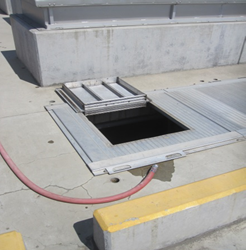
\includegraphics[scale=0.8]{SafetyFallProtection2}\\
\end{center}
\subsection{Noise}\index{Noise}
\begin{itemize}
\item Noise as a hazard is sound that is especially loud or impacting. 
\item A wastewater treatment plant has equipment that produces high noise levels both continuously and intermittently. 
\item As such, it is important to be aware of this hazard and to take preventive steps to reduce exposure to damaging noise levels by wearing effective hearing protection and to minimize the duration of the exposure to the noise.
\end{itemize}

\subsection{Electrical Hazards}\index{Electrical Hazards}
\begin{itemize}
\item Ordinary 120-V electricity can be fatal; most wastewater facility electrical systems operate at 120 to 4000 V or more.  
\item All voltages should be considered dangerous and potentially life threatening.  
\item Safe working rules and practices that should be followed when working on electrical systems
\item Before working on an electrical system, perform a job hazard analysis to determine any potential hazards and methods of abating those hazards
\end{itemize}

\subsection{Trenching \& Excavation Hazards}\index{Trenching \& Excavation Hazards}
\begin{itemize}
\item Trenching and excavation related to construction and repair activities are common to wastewater operations.  
\item These hazards include: cave-ins or trench collapses, falls and falling loads, mobile/construction equipment accidents and hitting utility lines.
\end{itemize}

\subsection{Rotating and Moving Equipment}\index{Rotating and Moving Equipment}

\begin{itemize}
\item All rotating and moving equipment should be guarded. 
\item The best method for preventing machinery-related injuries is through use of equipment guards enforced through engineering and administrative controls.   
\item The best way to prevent this type of injury is to install point-of-operation guards that prevent contact with ingoing nip points, pinch points, rotating parts, flying chips, and sparks.
\end{itemize}
\begin{center}
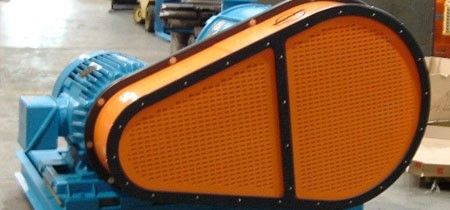
\includegraphics[scale=0.6]{SafetyMachineGuarding}\\
\end{center}

\subsection{Heat Stress}\index{Heat Stress}
\begin{itemize}
\item Heat stress falls into two categories: heat illness and heat stroke. 
\item Both are serious conditions and should not be taken lightly. 
\item Heat stress can result from: 
\begin{itemize}
\item High temperature and humidity, dehydration from low fluid consumption
\item Direct sun exposure (with no shade) or extreme heat, 
\item Limited air movement (no breeze or wind), 
\item Physical exertion, Use of bulky protective clothing and equipment, 
\item Poor physical condition or ongoing health problems, 
\item Some medications
\item Pregnancy
\end{itemize}
\end{itemize} 

\subsection{Biohazards}\index{Biohazards}
\begin{itemize}
\item Biological hazards including pathogens, associated with wastewater treatment may result from either direct contact with wastewater or through air dispersion.
\item Biohazards associated with wastewater treatment include:
\begin{itemize}
\item Bacteria - including \textit{E. coli, salmonella, legionella, shigellosis, cholera and typhus}.
\item Viruses such as hepatitis.
\item Fungi - these include aspergillus which can grow in compost.
\item Parasites - Giardia and roundworm are a couple of examples.
\end{itemize}
\item Practices to safeguard operators and other treatment plant workers include:
\begin{itemize}
\item Wash hands thoroughly with soap and water frequently.
\item Avoid touching face, mouth, eyes, nose, genitalia, or open sores and cuts while
working in the wastewater treatment environment.
\item Washing hands before eating, drinking, or smoking and before and after using the
bathroom.
\item Eating in designated areas.
\item Using barriers between skin and surfaces exposed to wastewater.
\item Keeping wounds covered with clean, dry bandages.
\item Changing into clean work clothing on a daily basis and reserve footgear for use at
worksite.
\item Not wearing work clothes home or outside the work environment.
\item Use gloves to prevent skin abrasion.
\end{itemize}
\item Periodic training on standard hygiene practices for wastewater treatment workers should be conducted by qualified safety and health professionals.
\item Appropriate PPE  including goggles, splash-proof face shields, respirators, liquid-repellent coveralls, and gloves should be provided.
\item Ensuring all employees are up-to-date on the mandated or recommended immunizations.
\end{itemize}

\subsection{Material Handling Ergonomics}\index{Material Handling Ergonomics}
\begin{itemize}
\item Wastewater operators are potentially subject to risk of musculoskeletal injuries associated with handling heavy or unwieldy objects including tools and supplies as part of their daily work routine.
\item The risk and severity of these injuries can be mitigated through utilizing proper ergonomic techniques which include:
\begin{itemize}
\item Use mechanical means (e.g. hand trucks, pushcarts, etc.) when possible for heavier or awkward loads.
\item It is easier and safer to push than to pull.
\item Keep loads as close to the body as possible and do not twist while lifting, carrying, or setting down a load. Nose, shoulders, hips, and toes should all be facing the same direction.
\item Minimize reaching.
\item As a general rule, bend at the knees, not the hips.
\item Get help when needed. Do not lift or carry things you don’t feel comfortable with, no matter how light the load.
\item Plan ahead for all parts of the lift: lifting, carrying, and setting down.
\item Use personal protective equipment where needed, such as gloves with good grip and steel-toed boots where appropriate.
\item Implement rest breaks and job rotation for frequent and/or heavy lifting.
\end{itemize}
\end{itemize}



\section{Safety Practices}\index{Safety Practices}


\subsection{Lockout - Tagout (LOTO)}\index{Lockout - Tagout (LOTO)}

When conducting routine inspections, repairs and maintenance activities, requires meeting the mandates of \hl{Occupational Safety  Hazard Administration(OSHAs) Lock-Out/Tag-Out (LOTO) program}\\
which is designed to prevent injury or fatalities.  It involves preventing an equipment from accidentally starting up and release of all stored energy.  Hazardous energy sources include: 
\begin{itemize}
\item Electrical 
\item Mechanical
\item Hydraulic
\item Pneumatic 
\item Chemical 
\item Thermal  
\item Other energy
\end{itemize}

The LOTO involves established and documented procedures specific to an equipment or machinery.  It typically comprises of:\\
\begin{itemize}
\item Notifying affected employees
\item Stopping and isolating the equipment
\item Releasing stored energy
\item Verification of the isolation and de-energization
\item Placing lock-out devices which use a positive means such as a lock, either key or combination type, to hold an energy isolating device in the safe position and prevent the energizing of a machine or equipment
\item Appropriately tagging the devices to indicate its non-operation and that it may not be operated until the tagout device is removed
\end{itemize}

\subsection{Personal Protective Equipment (PPE)}\index{Personal Protective Equipment (PPE)}
Employees depend on personal protective equipment to protect themselves from hazards and perform daily duties. PPE includes but is not limited to safety glasses, face shields, hard hats, gloves, foot protection, and durable and disposable chemical-protective clothing. Respirators and fall protection might also be required. However, respirators and fall protection fall under separate OSHA standards. \\

\subsection{Confined Space Entry}\index{Confined Space Entry}
OSHA defines a confined space as an area that:
\begin{itemize} 
\item is large enough and so configured that an employee's body can enter and perform assigned work
\item has limited or restricted means for entry or exit; and
\item is not designed for continuous employee occupancy.
\end{itemize}
Potentially dangerous conditions which can exist in confined spaces include: 
\begin{itemize}
\item Oxygen level: Some gasses are heavier than air and so will fill up a confined space, which forces oxygen out.  The oxygen concentration must not fall below 19.5\% at any time.  In plants where pure oxygen is used there is a potential hazard due to high the oxygen concentration.  Oxygen concentration greater than 23\% increases the risk of ignition and fire
\item Explosive conditions:  Many gasses are explosive when present in certain ratios with oxygen. These ratios are defined by the upper explosive limit(UEL) and the lower explosive limit (LEL).  The minimum concentration of a particular combustible gas or vapor necessary to support its combustion in air is defined as the Lower Explosive Limit (LEL) for that gas. Below this level, the mixture is too “lean” to burn. The maximum concentration of a gas
or vapor that will burn in air is defined as the Upper Explosive Limit (UEL). Above this level, the mixture is too “rich” to burn.  The range between the LEL and UEL is known as the flammable range for that gas or vapor.  
\item Toxic conditions:  This condition could potentially exist due to the presence of gasses such as carbon dioxide, chlorine and hydrogen sulfide.
\item Engulfment by liquids
\item Electrical hazards
\item Mechanical Hazards associated with equipment including mixers
\end{itemize}

A permit-required confined space is defined as a confined space that:
\begin{itemize} 
\item contains or has a potential to contain a hazardous atmosphere
\item contains a material that potentially could engulf an entrant
\item has an internal configuration that could trap or asphyxiate an entrant through inwardly converging walls or a floor that slopes downward and tapers to a smaller cross-section
\item contains any serious safety or health hazard
\end{itemize}





